The second hypothesis is finding out which environmental factors are the best predicters of temperature for Salt Lake City. According to \cite{epa_utah}, higher temperature results in either more or less percipitation and higher frequency of storms. Using this information, this study performs a multilinear regression of Temperature against percipitation, number of thunderstorms per month, and minutes of sunlight per month. Minutes of sunlight was added because it is the most obvious indicator of temperature. Unfortunately, sunlight data was only recorded from 1965 to 2004, so we restrict our study down to this range. Furthermore, our data shrinks from 479 months to 322 months because either temperature, number of thunderstorms, or percipitation have missing values in these years.

\begin{figure}
  \centering
  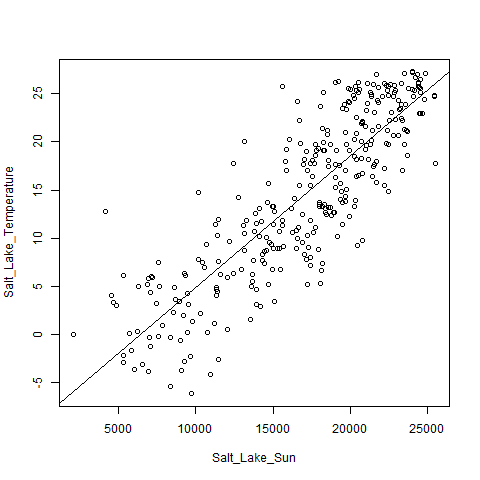
\includegraphics[width=15cm]{../data/img/Temp_vs_sun.PNG}
  \caption{Salt Lake City Temperature versus Sun}
  \label{fig:temp_vs_sun}
\end{figure}

\begin{figure}
  \centering
  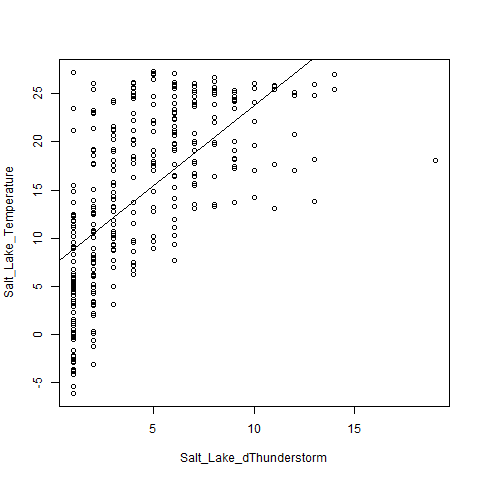
\includegraphics[width=15cm]{../data/img/Temp_vs_dThunderstorm.PNG}
  \caption{Salt Lake City Temperature versus Days of Thunderstorms}
  \label{fig:temp_vs_dthunderstorms}
\end{figure}

\begin{figure}
  \centering
  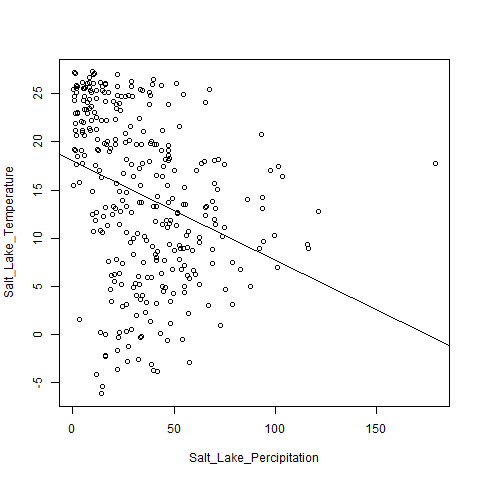
\includegraphics[width=15cm]{../data/img/Temp_vs_Percipitation.PNG}
  \caption{Salt Lake City Temperature versus Percipitation}
  \label{fig:temp_vs_percipitation}
\end{figure}

Firstly, to get a sense of data trends, we observe temperature data by each dependent variable with a line of best fit. As expected, there is a strong positive correlation between minutes of sunlight and temperature in Figure \ref{fig:temp_vs_sun}. By inspection, there also happens to be a decent positive correlation between number of thunderstorms and temperature in Figure \ref{fig:temp_vs_dthunderstorms}. However, the correlation between percipitation and temperature is negative in Figure \ref{fig:temp_vs_percipitation}, which is expected in some regions as stated in \cite{epa_utah}. In addition, if we want to obtain the best multilinear regression to predict temperature, it is best to use parameters that are not highly correlated with each other, as adding additional highly correlated variables adds to model complexity without much benefit. Figure \ref{fig:correlation_plot} suggests that the dependent variables sunlight, days of thunderstorm, and percipitation are not highly correlated so they are good initial choices.

\begin{figure}
  \centering
  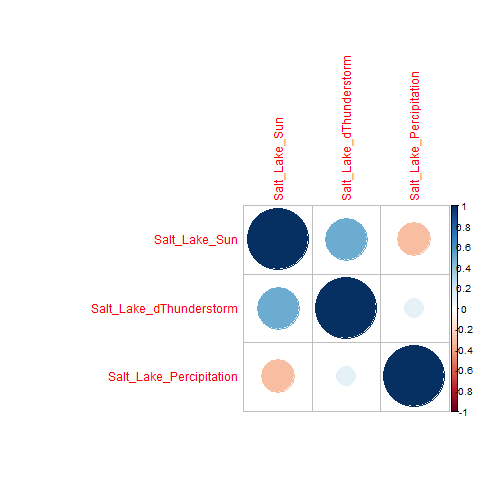
\includegraphics[width=10cm]{../data/img/correlation_plot.PNG}
  \caption{Correlation plot of chosen dependent variables}
  \label{fig:correlation_plot}
\end{figure}

TODO: TALK ABOUT PERFORMING REGRESSION WITH SUN, SUN/DTHUNDER, AND SUN/DTHUNDER/PERCIPITATION... 

\begin{table}[ht]
 \begin{centering}
 \begin{tabular}{|c|c c|} 
 \hline
 $$ & $\Delta T$ Salt Lake City & $\Delta T$ Rye Patch \\ [0.5ex] 
 \hline\hline
  $\mu$ & 1.1229 & 0.1317 \\ 
 \hline
 $\sigma$ & 1.9765 & 1.9226 \\
  \hline
 $n$ & 487 & 487 \\ 
  \hline
 $P_{Shapiro}$ & 0.0166 & 0.0003 \\ 
 \hline
 \end{tabular}
 \caption{Temperature Difference Statistics}
 \label{tab:temp_diffs}
 \end{centering}
\end{table}

\begin{table}[ht]
 \begin{centering}
 \begin{tabular}{|c|c|} 
 \hline
  $t$ & -16.46 \\ 
 \hline
 $df$ & 486 \\
  \hline
 $P$ & $2.2 \times 10^{-16}$ \\ 
  \hline
 Conf. Interval & $(-1.1095, -0.8728)$ \\ 
 \hline
 \end{tabular}
 \caption{Paired t Test Results for $\Delta T$}
 \label{tab:t_test_results}
 \end{centering}
\end{table}